\documentclass{beamer}
\usepackage[utf8]{inputenc}
\usepackage{tikz}
\usetikzlibrary{patterns}
\usetikzlibrary{shapes.geometric}
\usetikzlibrary{calc}
\usetikzlibrary{automata,positioning}

\usepackage{array}
\usepackage{chemfig}
\usepackage{multirow}
\usepackage{caption}
\usepackage{amsmath}
\usepackage{amssymb}
\usepackage[cal=boondoxo]{mathalfa} 
\usepackage{enumitem}
\usepackage{lastpage}
\usepackage{tcolorbox}
\usepackage{siunitx}
\usepackage[european, straightvoltages, RPvoltages]{circuitikz}


\usepackage{multicol}
\usepackage{eqnarray}


\usepackage{esvect}
\usepackage{siunitx}
 \sisetup{
    detect-all,
    output-decimal-marker={,},
    group-minimum-digits = 3,
    group-separator={~},
    number-unit-separator={~},
    inter-unit-product={~}
} %setup pour SIunitx


\title{Corrections d'activités}
\author{Rémy Rosalie}
\date{Mai 2024}

\begin{document}

\maketitle
\begin{frame}{TP : Rendement d'une cellule photoélectrique}
\begin{minipage}{\linewidth}
\textbf{Question 1 ) Représenter la chaîne énergétique du panneau photovoltaïque, en identifiant les puissances reçues, perdues et utiles, et en nommant la forme d'énergie associée.}
\end{minipage}\\
\begin{center}
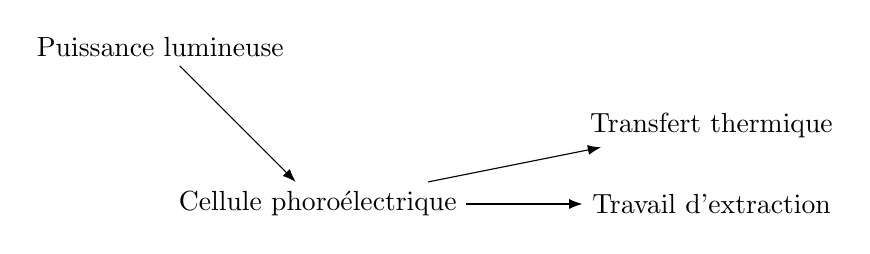
\begin{tikzpicture}
	\node (S) at (0,0){Cellule phoroélectrique};
	\node (L) at (-2,2){Puissance lumineuse};
	\node (H) at (5,1){Transfert thermique};
	\node (E) at (5,0){Travail d'extraction};
	\draw[-Latex] (L) to (S);
	\draw[-Latex] (S) to (H);
	\draw[-Latex] (S) to (E);
\end{tikzpicture}
\end{center}
\end{frame}

\begin{frame}{TP : Rendement d'une cellule photoélectrique}
\begin{minipage}{\linewidth}
\textbf{Question 2 ) Commenter les courbes du Doc. 2.}\\
\end{minipage}

\begin{minipage}{.5\linewidth}
	
\includegraphics[width=\linewidth]{Ressources/TSPE_C16_Act2_fig2.png}
\end{minipage}\begin{minipage}{.5\linewidth}
	On constate que l'intensité est stable lorsque la tension augmente jusqu'à une certaine valeur après laquelle elle commence à chuter fortement jusqu'à 0.\\
	De même ma puissance augmente de manière linéaire jusqu'à une valeur de tension pour laquelle elle va chuter vers 0.\\
	Cela crée donc une valeur optimale de puissance que l'on appelle "valeur crête".
\end{minipage}
\end{frame}

\begin{frame}{TP : Rendement d'une cellule photoélectrique}
\begin{minipage}{\linewidth}
\textbf{Question 3 ) Tracer la caractéristique $I=f(U)$, puis la courbe $P=f(U)$ de la cellule. Déterminer la puissance maximale de la cellule, appelée puissance de crête.}\\
\end{minipage}

\begin{minipage}{.5\linewidth}
	%
\includegraphics[width=\linewidth]{Ressources/TSPE_C16_Act2_fig2.png}
\end{minipage}\begin{minipage}{.5\linewidth}
\end{minipage}

\begin{minipage}{.5\linewidth}
	%
\includegraphics[width=\linewidth]{Ressources/TSPE_C16_Act2_fig2.png}
\end{minipage}\begin{minipage}{.5\linewidth}
\end{minipage}

\end{frame}






\begin{frame}{TP : Électroraffinage du cuivre}
	\begin{minipage}{\linewidth}
	\textbf{Question 1 ) Proposer une définition du mot électroraffinage}\\

	On peut le décomposer en deux partie : "\emph{électro}" faisant référence à l'électricité, puis "\emph{raffinage}" qui fait référence à une purification. Ainsi "électroraffinage" fait désigne une technique utilisant l'électricité  pour purifier des métaux.
	\end{minipage}
	\end{frame}

\begin{frame}{TP : Électroraffinage du cuivre}
	\begin{minipage}{\linewidth}
	\textbf{Question 2 ) Qu'observe-t-on au niveau des électrodes ?}\\
	On remarque que l'électrode branchée à la borne négative du générateur a un aspect de moins en moins lisse.  L'électrode branchés que la borne positive semble moins épaisse.
	\end{minipage}
	\end{frame}
	
\begin{frame}{TP : Électroraffinage du cuivre}
\begin{minipage}{\linewidth}
\textbf{Question 3 ) Pourquoi cette électrolyse est-elle appelée : \emph{électrolyse à anode soluble} ?}\\

Lors de cette électrolyse, la compensation des charges dans la solution fait que des atomes ce cuivre solide de l'électrode positive réagissent pour libérer des électrons en solution. On a donc une oxydation qui se met en place à cette électrode de formule $$Cu(s) \rightarrow Cu^{2+}(aq) + 2e^{-}$$
L'anode (siège de l'oxydation) va donc se dissoudre dans la solution. 
\end{minipage}
\end{frame}

\begin{frame}{TP : Électroraffinage du cuivre}
\begin{minipage}{\linewidth}
\textbf{Question 4 ) Compléter le schéma}
\begin{center}
	
\includegraphics[width=.7\linewidth]{Ressources/TSPE_C16a_Electroraffinage_Fig1.png}
\end{center}
\end{minipage}
\end{frame}


\begin{frame}{TP : Électroraffinage du cuivre}
\begin{minipage}{\linewidth}
\textbf{Question 5 ) En rappelant les réactions ayant lieux à l’anode et à la cathode, écrire les deux demi-équations électroniques mises en jeu.}\\
\textbf{Anode :} Oxydation : $$Cu(s) \rightarrow Cu^{2+}(aq) + 2e^{-}$$
\textbf{Cathode :} Réduction : $$Cu^{2+}(aq) + 2e^{-} \rightarrow Cu(s)$$
\end{minipage}
\end{frame}


\begin{frame}{TP : Électroraffinage du cuivre}
\begin{minipage}{\linewidth}
\textbf{Question 6 ) A quelle électrode doit-on mettre le métal brut ?}\\
Le métal brut ($Cu(s)$)  doit se retrouver à l'anode puisque c'est à cette électrode qu'il est "utilisé".
\end{minipage}
\end{frame}

\begin{frame}{TP : Électroraffinage du cuivre}
\begin{minipage}{\linewidth}
\textbf{Question 7 ) A quelle électrode récupère-t-on le cuivre métallique ?}\\
Le cuivre métallique vient se déposer sur la cathode.
\end{minipage}
\end{frame}

\begin{frame}{TP : Électroraffinage du cuivre}
\begin{minipage}{\linewidth}
\textbf{Question 8 ) Quel est l'intérêt de l'électrolyse ?}\\
Cette méthode permet de transformer des ions métalliques en solution en métal à l'état solide. Elle permet ainsi de purifier des solutions ou des métaux. Il faut cependant "sacrifier" un autre métal.
\end{minipage}
\end{frame}

\begin{frame}{TP : Électroraffinage du cuivre}
\begin{minipage}{\linewidth}
\textbf{Question 9 ) Comment varie la concentration en ions cuivre dans la solution ?}\\
Dans notre cas, la concentration des ions cuivre en solution ne varie pas puisqu'il y a autant d'ions libérés en solution par l'anode que d'ions consommés à la cathode
\end{minipage}
\end{frame}

\begin{frame}{TP : Électroraffinage du cuivre}
\begin{minipage}{\linewidth}
\textbf{Question 10 ) Déterminer la quantité de matière d’électrons échangés $n_{e^-}$ pendant l’électrolyse.}\\
\vspace{5cm}
\end{minipage}
\end{frame}

\begin{frame}{TP : Électroraffinage du cuivre}
\begin{minipage}{\linewidth}
\textbf{Question 11 ) Quel est le lien entre la quantité de charge $Q$, l’intensité du courant $I$ et la durée de l’électrolyse $\Delta t$ ?}\\
On sait que $I=\dfrac{Q}{\Delta t}$ donc $$ Q = I \cdot \Delta t$$
\end{minipage}
\end{frame}

\begin{frame}{TP : Électroraffinage du cuivre}
\begin{minipage}{\linewidth}
\textbf{Question 12 ) Quel est le lien entre la quantité de charge Q, la quantité de matière d’électrons échangés $n_{e^-}$ et la constante de Faraday ?}\\
On sait que $Q = n_{e^-} \cdot \mathcal{F}$
\end{minipage}
\end{frame}

\begin{frame}{TP : Électroraffinage du cuivre}
\begin{minipage}{\linewidth}
\textbf{Question 13 ) Calculer la masse maximale de cuivre déposé}\\
Puisque $Q = I \cdot \Delta t$ et $Q = n_{e^-} \cdot \mathcal{F}$, on peut déterminer la quantité d'électrons maximale transférée :
$$ I \cdot \Delta t =  n_{e^-} \cdot \mathcal{F}$$
$$ n_{e^-} = \dfrac{I \cdot \Delta t}{\mathcal{F}} $$
$$ n_{e^-} = \dfrac{I \cdot \Delta t}{N_A \cdot e} $$
\fbox{AN} : $ n_{e^-} = \dfrac{0,1 \cdot 15 \times 60}{\num{6,02E23} \cdot \num{1,60E-19}} = \SI{1,50E-3}{\mole}$\\
Sachant que chaque entité de cuivre déposé nécessite un transfert de deux électrons, on aura donc \SI{7,50E-4}{\mole} de cuivre déposé. Soit \SI{47,5}{mg}.
\end{minipage}
\end{frame}

\begin{frame}{TP : Électroraffinage du cuivre}
\begin{minipage}{\linewidth}
\textbf{Question 14 ) Analyser le rendement de l'électrolyse}\\
\vspace{5cm}
\end{minipage}
\end{frame}

\end{document}